\documentclass[11pt,openright,twoside]{report}
\usepackage[utf8]{inputenc}
\usepackage[portuguese, english]{babel}
\usepackage{graphicx}
\usepackage{hyperref}
\usepackage{natbib}

\title{\textbf{Relatório - Ambientes Gráficos em Linux}}
\author{Turma 1 - Diogo Ferreira e Luís Leira\\\vspace{3cm}
Universidade de Aveiro - Laboratórios de Informática}
\date{\today}
\begin{figure}
 \center
 
\includegraphics[scale=1.5]{ua_logo.png}
\end{figure}


\begin{document}

\selectlanguage{portuguese}
\maketitle
\tableofcontents

\part{Apresentação}


\chapter{Resumo}
\paragraph{  }Neste trabalho são analisados com detalhe alguns ambientes gráficos e gestores de janelas do sistema Linux, entre os quais: \textit{KDE, Ubuntu Unity, XFCE4, LXDE, E17, xmonad} e \textit{awesome}.

  
 \textbf{ Resumo dos ambientes gráficos usados:}

  \begin{description}


  \item[KDE] \hfill \\
  Totalmente personalizável, efeitos gráficos bastante avançados. Interface acessível e intuitiva. Aconselhado a utilizadores que dão privilégio ao aspeto gráfico e com hardware que suporte este ambiente, visto que é ainda algo pesado para computadores limitados comparativamente com as opções abaixo descritas.
  
  \item[Unity] \hfill \\
  Sistema de eleição da comunidade de Linux. Interface gráfica sólida e facilidade no seu uso, grande comunidade e elevado número de aplicações disponíveis. Aconselhado a utilizadores regulares que necessitam de recursos normais para o dia-a-dia e de fácil acessibilidade. No entanto, o maior problema são os recursos que necessita, pois foi o que necessitou de maior memória Ram e CPU nos nossos testes.
  
 \item[XFCE4] \hfill \\
  Estável e personalizável. Aconselhado à maioria dos utilizadores, especialmente os que procuram um sistema rápido.
  
  \item[E17] \hfill \\
  Interface original, inovador, leve e personalizável. Aconselhado a utilizadores que pretendem algo fora do comum e que possa ser moldado ao seu gosto.
  
  \item[LXDE] \hfill \\
   Baixo consumo de memória e CPU. É um sistema bastante leve e simples, similar ao XFCE.
  
    \end{description}
  
  \textbf{Resumo dos gestores de Janelas usados:}
  
  \begin{description}

  \item[Xmonad] \hfill \\
  Facilidade de uso e utilização de poucos recursos. Aconselhado a utilizadores que pretendem uma execução eficiente num computador mais limitado.
  
  \item[awesome] \hfill \\
  Rápido, baixo impacto na memória e CPU, personalizável. Aconselhado a utilizadores avançados que pretendem realizar tarefas computacionais com mais exigência.
 
  \end{description}

\chapter{Introdução}

\paragraph{  }O Linux {\it (\autoref{linux})} é um sistema operativo criado por Linux Torvalds em 1991 baseado no \textit{Unix}, com o objetivo de ser {\it open-source}, para que todos o pudessem usar e modificar livremente \cite{Linux}. No início, tinha um aspeto pouco prático para um utilizador regular, sendo necessário ter conhecimentos específicos para interagir com a máquina. No entanto, ao longo dos anos, foram desenvolvidas inúmeras soluções para resolver o seu problema de usabilidade, traduzidas em interfaces gráficas que facilitam a interação com o utilizador \cite{Ambientesgraficos}.

\begin{figure}
 \center
 
\includegraphics[scale=.07]{tux1.png}
 \caption{Logo do Linux. Fonte: http://clipartist.net}
 \label{linux}
\end{figure}


Neste trabalho pretendemos avaliar a utilidade e o desempenho de alguns ambientes gráficos para o sistema Linux. Iremos abordar os seguintes sistemas: {\it KDE, Ubuntu Unity, LXDE, E17, XFCE4, xmonad e awesome}.

Cada ambiente gráfico ou gestor de janelas oferece determinadas funcionalidades específicas para um tipo de utilizador diferente. O nosso objetivo é especificarmos as vantagens de cada um deles de acordo com um modelo de utilização. Para isso, testámos todos os sistemas referidos e fizemos uma análise aos mesmos.

O relatório encontra-se dividido pelos ambientes gráficos utilizados, por sua vez divididos em análises detalhadas do seu funcionamento.

\part{Desenvolvimento}

\chapter{Ambientes gráficos}
\paragraph{  }Temos como objeto de estudo os ambientes gráficos e gestores de janelas disponíveis para Linux. Estes, sendo possível serem alternados facilmente, tornam o sistema mais completo em funcionalidades e garantem que a comunicação do utilizador com a máquina seja mais fácil e prática. Por esta razão, consideramos importante o conhecimento da diversidade de interfaces gráficas existentes para que seja possível optar pela que melhor se adapta às características e necessidades desejadas. 

É através de janelas, ícones e menus que se dá normalmente esta interação do utilizador com o computador, tornando assim mais intuitiva a realização de tarefas e o uso de aplicações. Em suma, eles influenciam a usabilidade e produtividade de um sistema (\autoref{Amb}).

Os interfaces gráficos são sistemas completos, com um conjunto de aplicações, gestores de janelas e animações para o utilizador interagir com computador. Gestores de janelas são apenas sistemas que funcionam com janelas, quase sem animações, podendo alguns até funcionar sem rato \cite{Ambientesgraficos}.

\begin{figure}
 \center
 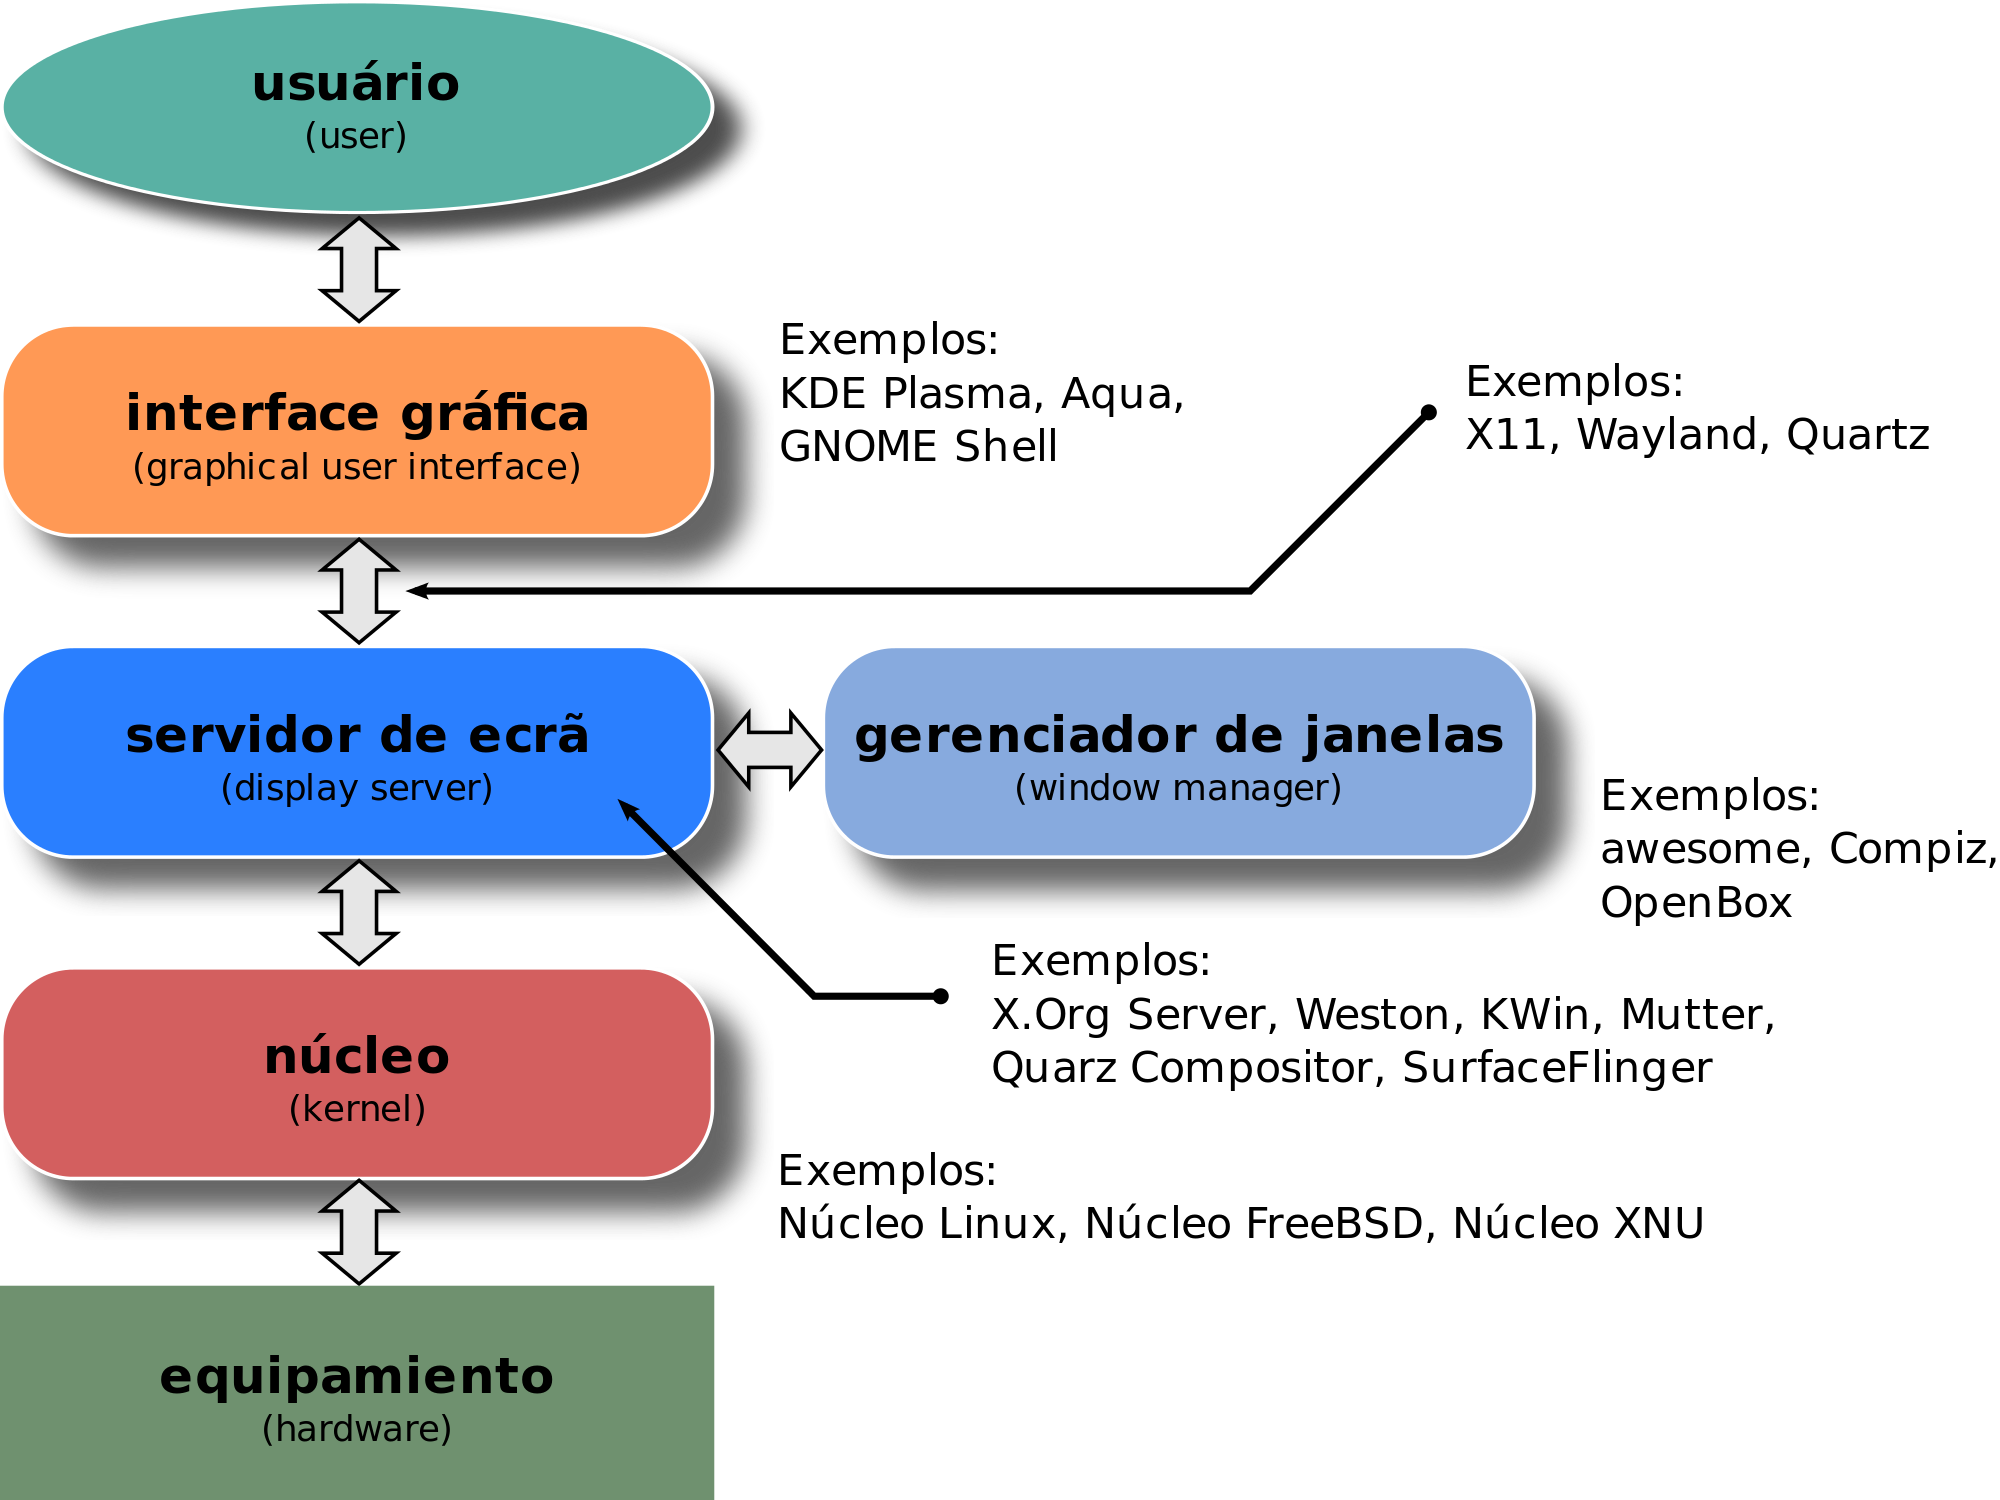
\includegraphics[scale=.175]{intgra.png}
 \caption{Esquema que explica a diferença sobre interfaces gráficas e gestores de janelas. Fonte: www.wikipedia.org}
 \label{Amb}
\end{figure}

\chapter{KDE}

\paragraph{  }KDE é um sistema criado por Matthias Ettrich em 1996 \cite{KDE}. O programador alemão tinha o intuito de criar uma interface gráfica unificada para sistemas \textit{Unix-like}. Inicialmente chamava-se \textit{Kool Desktop Environment}, mas em 2009 o nome foi alterado oficialmente para KDE. Ao longo dos anos, foi desenvolvido para ser um ambiente totalmente personalizável, permitindo ser ao gosto do utilizador.

Como tal, é dos ambientes gráficos de Linux mais utilizados e com uma grande comunidade, espalhada pelo mundo inteiro. O repositório de ficheiros pode ser encontrado em \url{https://en.opensuse.org/SDB:KDE_repositories}, atualizado diariamente. É abundante em recursos gráficos e em funcionalidades que facilitam a interação com o utilizador. Para além do desktop, KDE possui ainda uma vasta gama de aplicativos exclusivos que dão maior interesse ao sistema.

\begin{figure}
 \center
 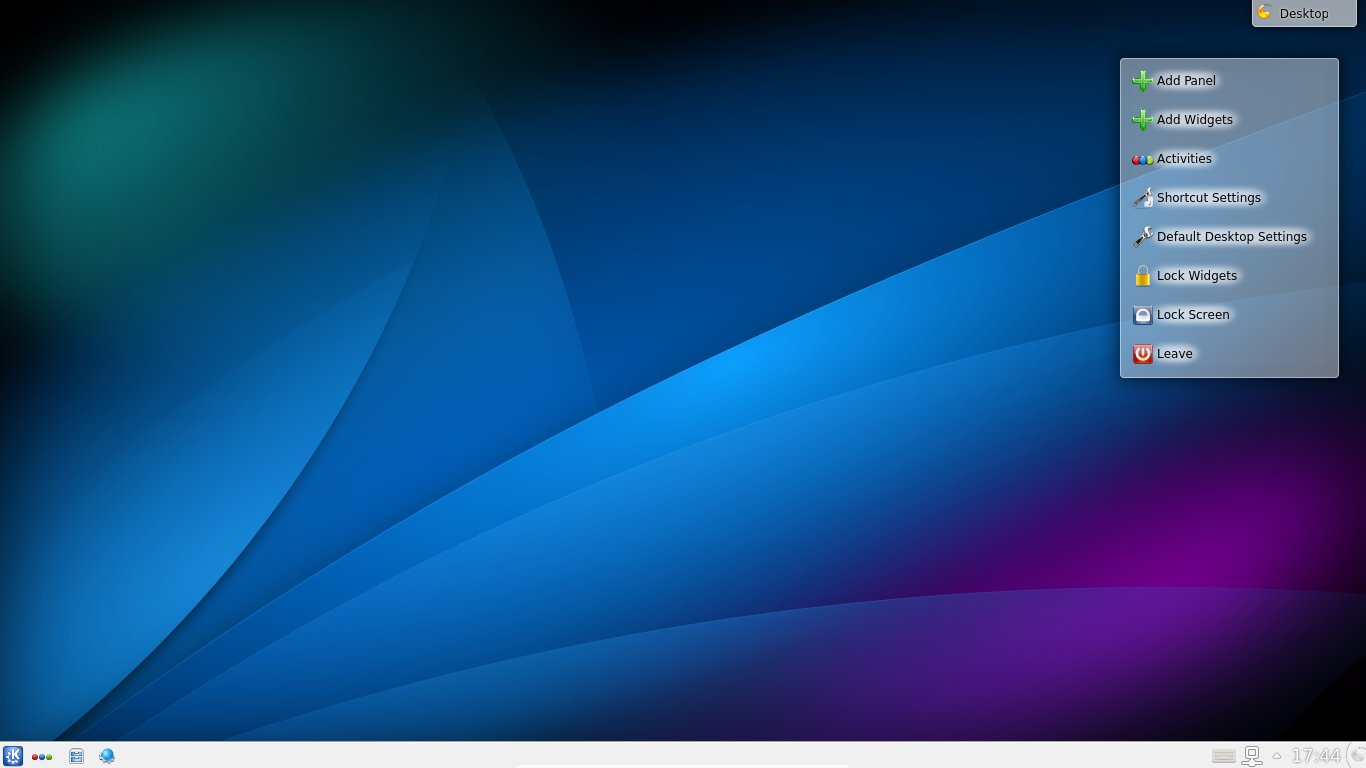
\includegraphics[scale=0.3]{kde.png}
 \caption{Ambiente de trabalho KDE.}
 \label{kde2}
\end{figure}

A interface do KDE tem algumas parecenças com o Windows. Como é totalmente personalizável, poderá diferir nos ícones, no papel de parede ou até nos botões do desktop. Quase tudo é personalizável: pode alterar-se a posição da barra de tarefas, dos ícones ou dos widgets \cite{InterfaceKDE}.

\begin{figure}
 \center
 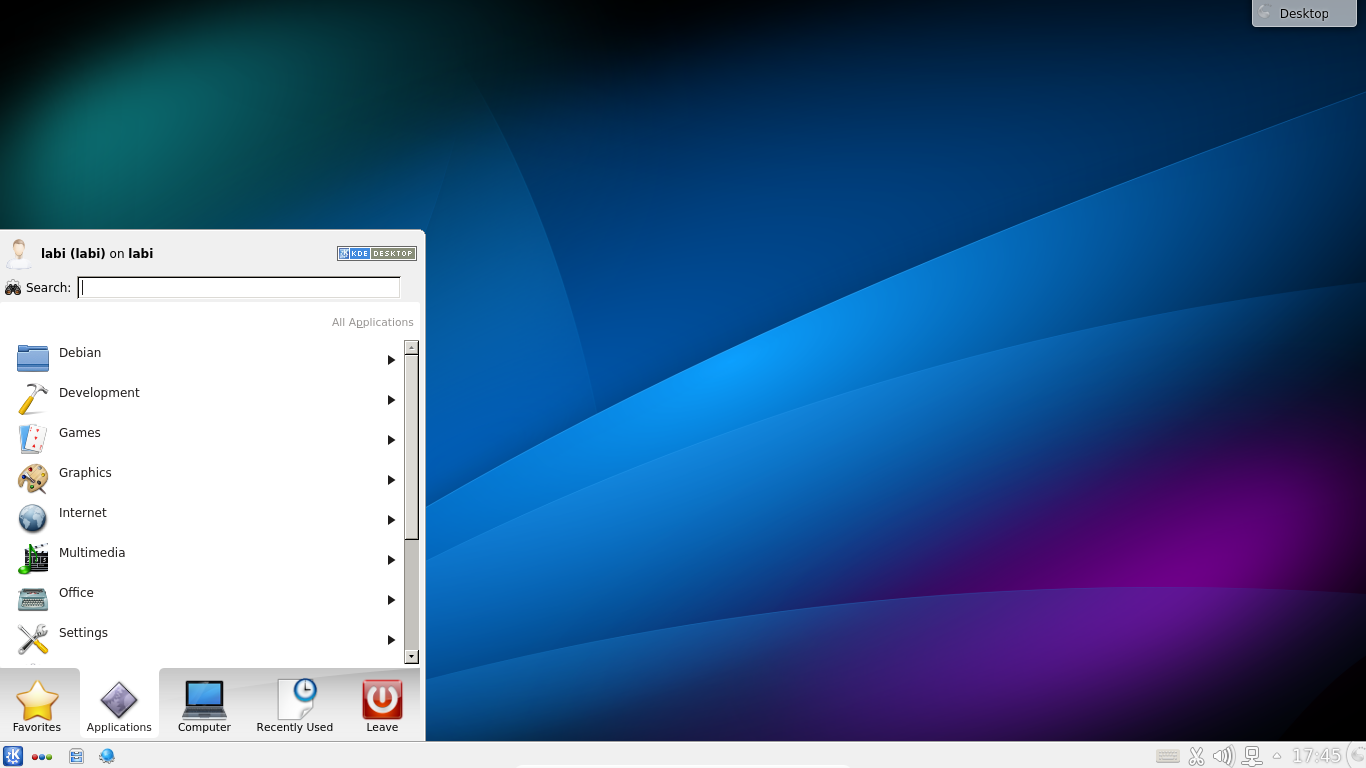
\includegraphics[scale=0.3]{mkde.png}
 \caption{Ambiente de trabalho KDE. Menu K com a opção de pesquisa ativada.}
 \label{kde}
\end{figure}

Na barra de tarefas podemos encontrar o menu K, parecido com o menu Iniciar do Windows 95 e 98 (\autoref{kde2}). Ao lado, temos os ícones de acesso rápido, personalizados pelo utilizador. Neste caso, apenas o Dolphin, o gestor de ficheiros \cite{dolphin}. As duas janelas do lado direito são referentes aos dois ambientes de trabalho virtuais que o sistema oferece. A seguir, podemos ver algumas aplicações do sistema e a data.

Os ficheiros no ambiente de trabalho estão dispostos na ordem que o utilizador entender. O papel de parede também é totalmente personalizável.

Abrindo o menu K (\autoref{kde}), é possível ter acesso às aplicações mais usadas divididas por géneros e às operações básicas do sistema. Ainda temos acesso à barra de pesquisa no topo do menu.

O gestor de ficheiros do KDE é, novamente, o Dolphin (pode ser alterado para o Konqueror, também pré-instalado), baseado novamente no Windows Explorer dos Windows. Do lado esquerdo temos acesso às pastas do diretório atual e acima, enquanto que na barra superior é possível escrever o diretório procurado ou ainda pesquisá-lo por ficheiro ou pasta.

No canto superior direto há um botão para adicionar e remover \textit{widgets} do \textit{desktop}.

No geral, a interface KDE é intuitiva para quem está habituado a utilizar Windows. Também tem a vantagem de ser totalmente adaptável conforme o utilizador.

O KDE divide as suas aplicações pré-instaladas em nove pacotes: Desenvolvimento, gràficos, produtividade, educação, internet, sistema, jogos, multimédia e uilitários. Dentro deles vêm as aplicações\cite{AplicacoesKDE}.

Há inúmeras aplicações desenhadas para KDE. Normalmente distinguem-se das outras pela sua primeira letra, que é um K. Alguns exemplos podem ser o Ktorrent, um servidor de transferência de ficheiros, o K3b, um gravador de \textit{DVD's, CD's} e ficheiros \textit{.ISO} e o famoso\textit{ Konqueror}, um gestor de ficheiros e \textit{web browser} (desde 2009 deixou de ser o gestor de ficheiros principal do KDE, passando a ser o \textit{Dolphin} \cite{dolphin}) (\autoref{konq}). É o sistema com maior número de aplicações desenhadas especificamente para a própria interface \cite{AppsKDE}.

\begin{figure}
 \center
 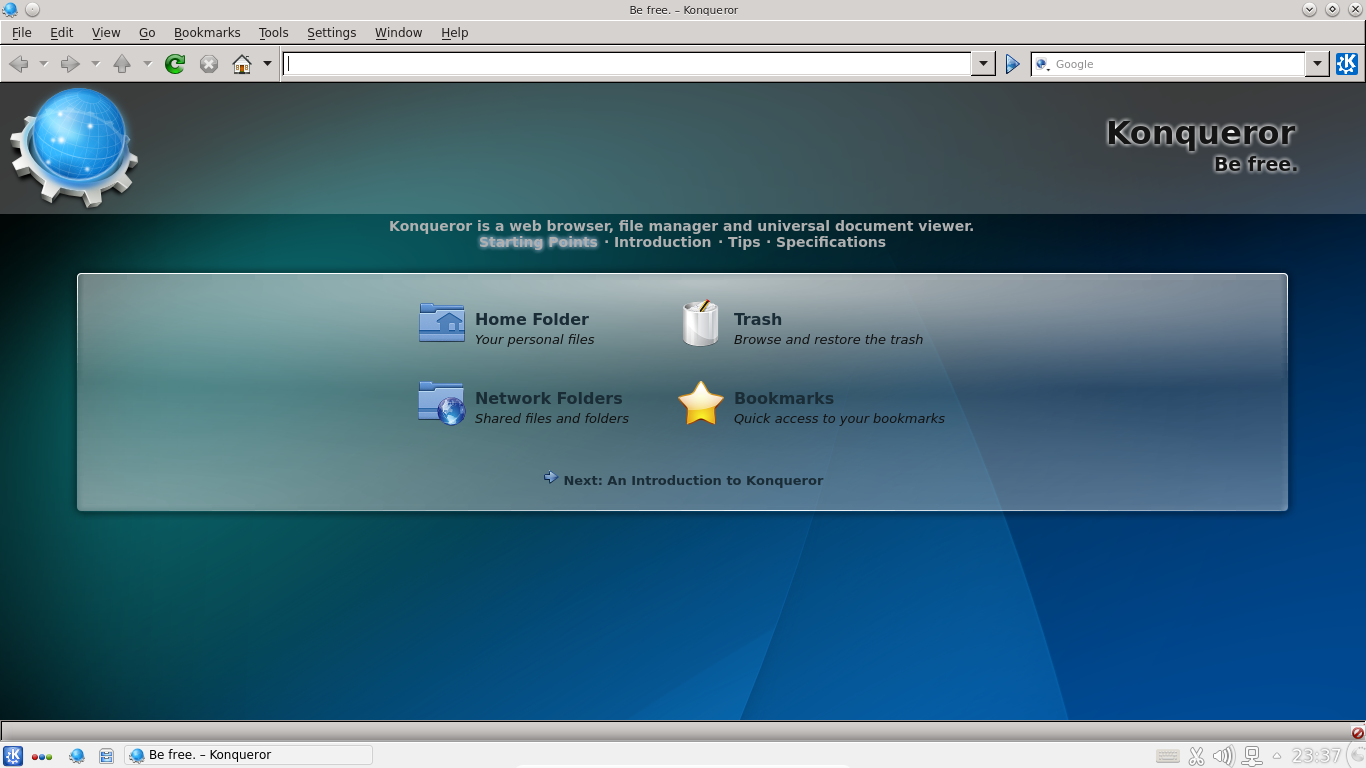
\includegraphics[scale=0.3]{konqueror.png}
 \caption{Web Browser Konqueror}
  \label{konq}
\end{figure}

Também os Widgets do KDE são bastante apelativos. Há de todo o tipo, e podem ser aplicados no \textit{Desktop}, na barra de tarefas ou mesmo sobrepondo as janelas já abertas.

Nos nossos testes de memória \cite{Memoriavirt}, vamos olhar para a componente \textit{RES} do processo do ambiente analisado.

O ambiente KDE utiliza uma quantidade de memória alta quando comparada com a maior parte das interfaces testadas (\autoref{memoria}). Tal como indica a figura (Processo Plasma-Desktop), utilizou 100 Mb da memória física disponível, sendo assim muito dispendioso no que diz respeito à memória Ram quando comparado com os outros ambientes. Na coluna da percentagem de CPU usada, o sistema utiliza 2,7\% do CPU, o que pode ser considerado um pouco elevado. No entanto, é compreensível que assim seja, pois é um sistema com bastantes efeitos gráficos integrados.

\begin{figure}
 \center
 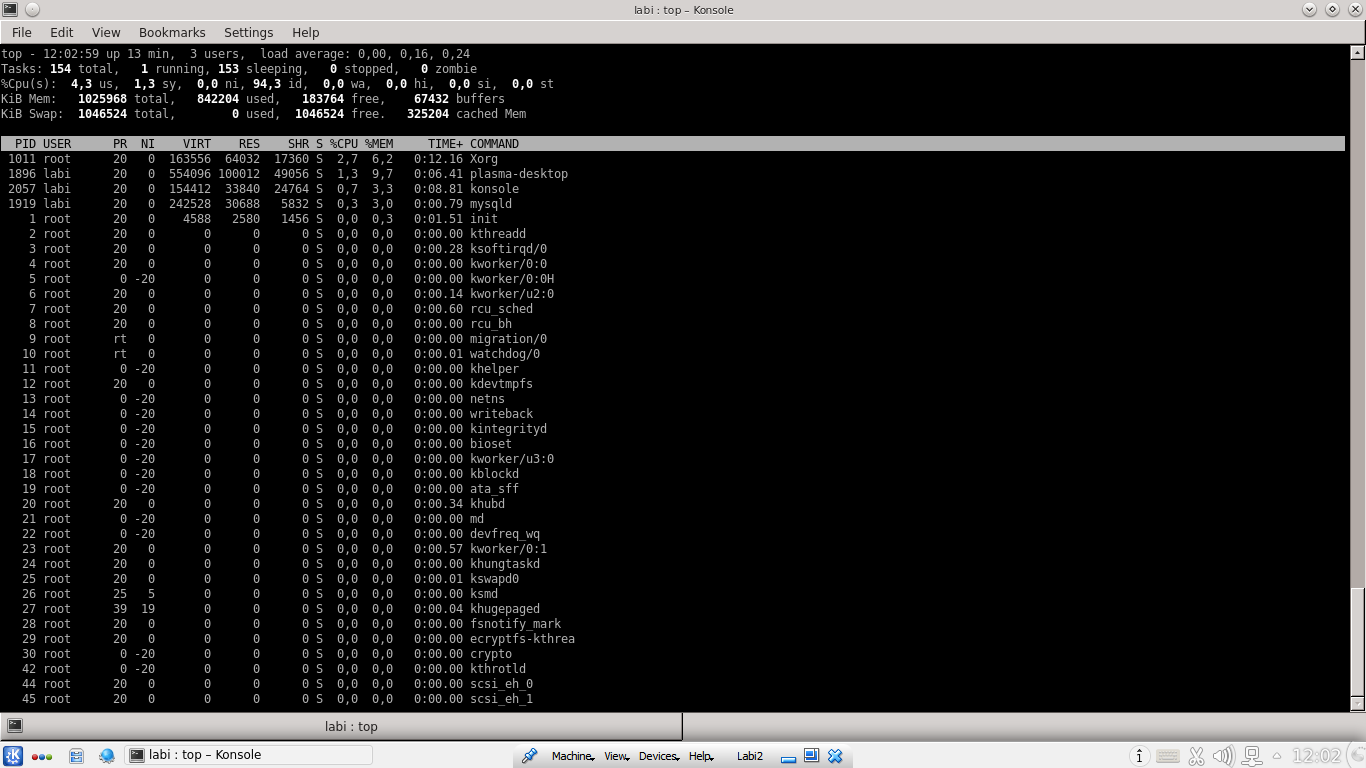
\includegraphics[scale=0.3]{memkde.png}
 \caption{Gestão de Memória no KDE. Dados baseados no segundo processo, \textit{plasma-desktop}.}
  \label{memoria}
\end{figure}



\chapter{Ubuntu Unity}

\paragraph{  }Em 2010 foi lançado o ambiente gráfico Unity, utilizado inicialmente no Ubuntu 10.10. Foi desenvolvido pela comunidade Ayatana e pela Canonical Ltd. É um ambiente que permite poupar espaço ao utilizador, introduzindo uma barra dinâmica lateral e uma superior, adaptando-se assim à necessidade de espaço dos \textit{laptops} \cite{Unity}.

Sendo alvo de um grande esforço comunitário por parte de todos os seus utilizadores, a sua qualidade evolui a um ritmo muito elevado. Portanto, a sua comunidade é um fator determinante e positivo no seu desenvolvimento. Os seus repositórios podem ser encontrados no link \url{http://www.ubuntuupdates.org/}.

É o sistema mais usual nos utilizadores Linux, pois para além de ser o pré-instalado no Ubuntu, é esteticamente avançado em relação à maioria dos ambientes.

A interface Unity é dinâmica e das mais elogiadas pelos utilizadores nos últimos tempos \cite{ApreciacaoUnity}. Com a sua barra lateral, permite ao utilizador de maneira simples e intuitiva chegar rapidamente à aplicação ou pasta desejada (\autoref{unity}). Pressionando um ícone na barra lateral, o ambiente inicia o programa com animações de \textit{Fade-in} e transparência (\autoref{menunity}).

\begin{figure}
 \center
 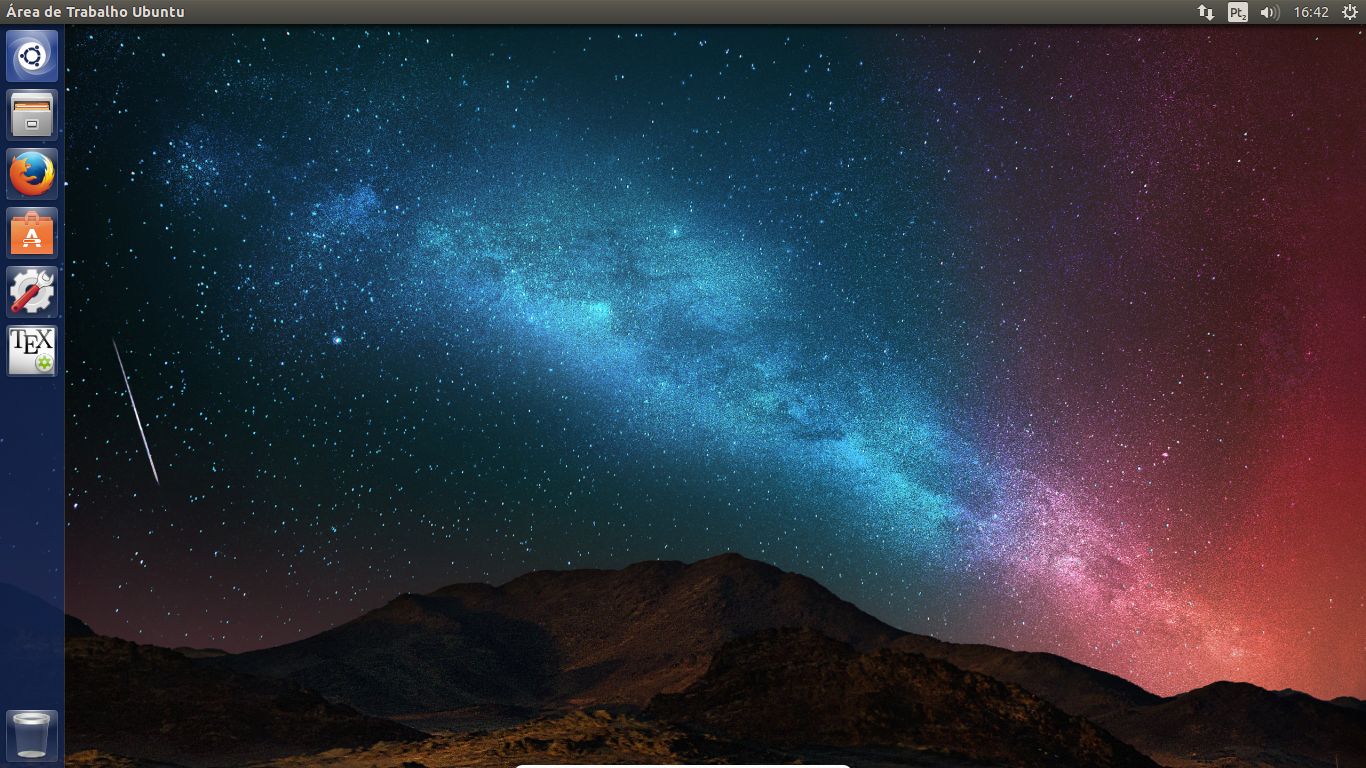
\includegraphics[scale=0.3]{unity.png}
 \caption{Ambiente de trabalho Unity, onde se pode ver a barra lateral e a barra superior.}
 \label{unity}
\end{figure}

\begin{figure}
 \center
 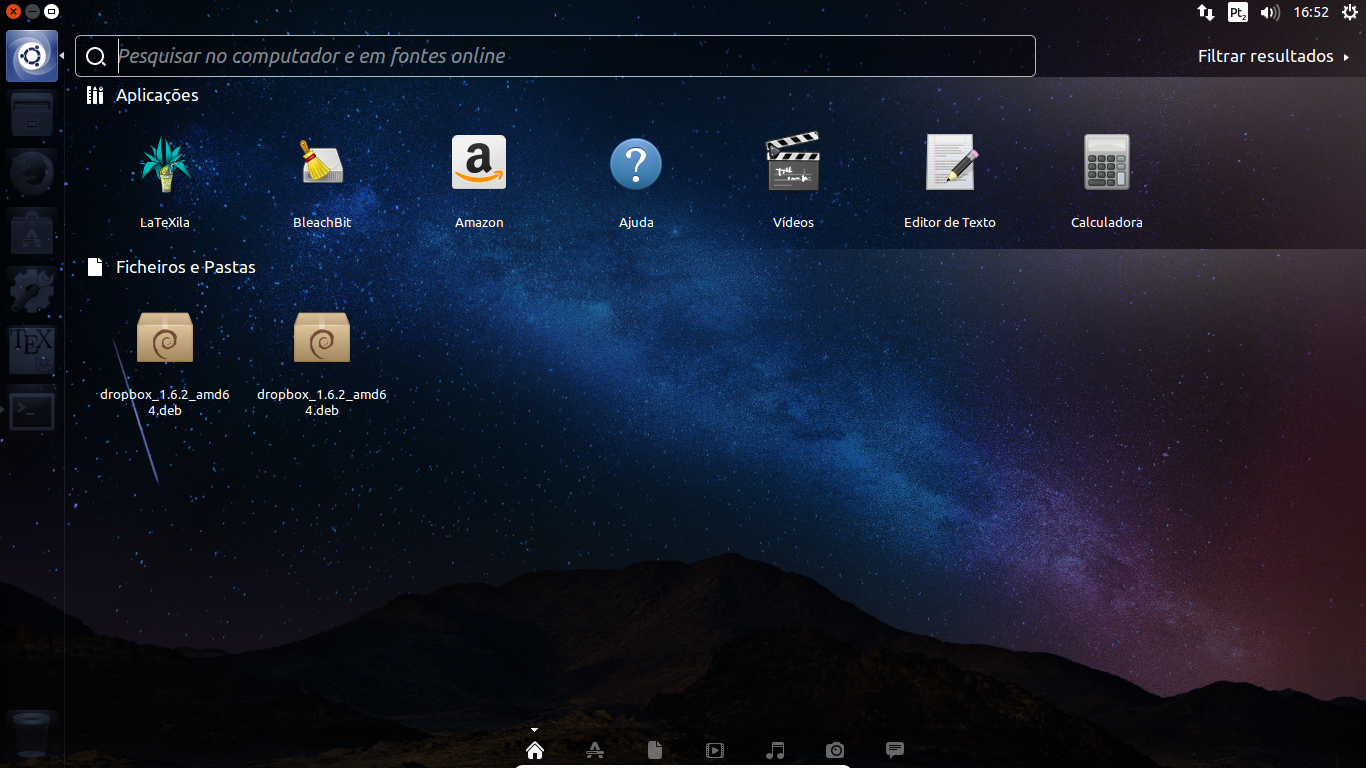
\includegraphics[scale=0.3]{unity2.png}
 \caption{Menu do Unity. Podemos reparar na imensa transparência na barra de tarefas, mesmo assim com os ícones completamente visíveis.}
 \label{menunity}
\end{figure}

No topo encontramos uma barra superior, que indica vários estados e definições do computador, assim como o nome de utilizador e as horas. Tem ainda vários sistemas dinâmicos de notificações.

Como o Unity é apenas um interface gráfico, iremos falar das aplicações pré-instaladas no Ubuntu, a sua "base". Há um elevado número delas específicas para esta distribuição, as quais poderão ser extremamente úteis \cite{AplicacoesUbuntu}.

O Geary, um leve e moderno cliente de e-mail, é um exemplo. Foi desenhado para se integrar perfeitamente com a interface Unity.

Também o Unity Tweak Tool é uma ferramenta muito usada para melhorar a aparência do software Unity. O VLC, o player de vídeo \textit{open-source} com mais downloads na plataforma Linux, também vem pré-instalado. Todas as aplicações disponíveis podem ser encontradas no \textit{Ubuntu Software Center}, uma interface gráfica com todos os repositórios disponveis para a plataforma.

Nos nossos testes relativamente ao consumo da memória por parte das interfaces, o Unity dispendeu quase 200 Mb de memória Ram (Processo compiz (\autoref{memuni})), o que pode inviabilizar a sua instalação em computadores mais antigos ou com menos memória Ram (especialmente quando usados para tarefas que necessitam de mais alguns recursos físicos do que o regular). Na verdade, é a principal desvantagem deste ambiente, que foi o que dispendeu mais memória física, quase o dobro do visto anteriormente.

Na utilização do CPU, o registo atingiu quase os 70\%, valor demasiado alto, podendo considerar-se um "pico" no registo dos recursos da interface. Tal deve-se aos efeitos ativados no momento em que a captura de ecrã foi utilizada, nomeadamente da barra lateral.

\begin{figure}
 \center
 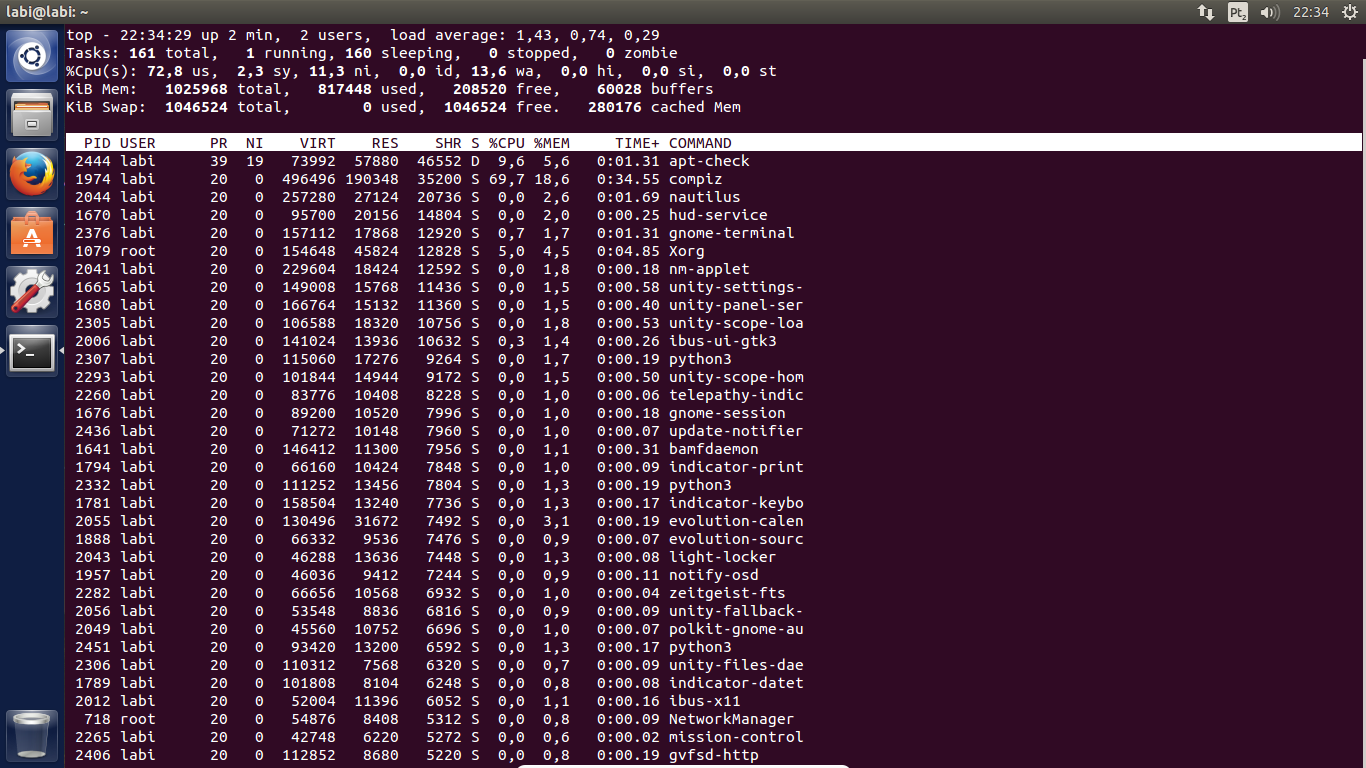
\includegraphics[scale=0.3]{memuni.png}
 \caption{Memória consumida pelo Unity. O processo usado foi o \textit{compiz}, novamente o segundo na lista de processos apresentados.}
 \label{memuni}
\end{figure}




\chapter{LXDE}

\paragraph{   }LXDE é um ambiente de desktop, que significa \textit{Lightweight X11 Desktop Environment} \cite{LXDE}. Foi criado por Hong Jen Yee em 2006, hacker asiático. Também ficou famoso pelo seu gestor de ficheiros \textit{PCManFM}, uma das referências principais do sistema.

É uma interface desenhada para ser leve, rápida e económica, mas completa, ideal para notebooks e computadores antigos com pouca capacidade de processamento. Foi desenhado em C/C++ e corre em sistemas baseados em Unix.

O sistema tem uma comunidade ativa desde o seu lançamento e os seus repositórios estão no link \url{http://git.lxde.org/}. No entanto, pela sua extrema facilidade de uso e existência de ambientes gráficos mais desenvolvidos esteticamente, não há muitas alternativas no que toca ao seu suporte.

A interface do LXDE é bastante simplista (\autoref{lxde}). Conta com a usual barra de tarefas, já vista no KDE.

\begin{figure}
 \center
 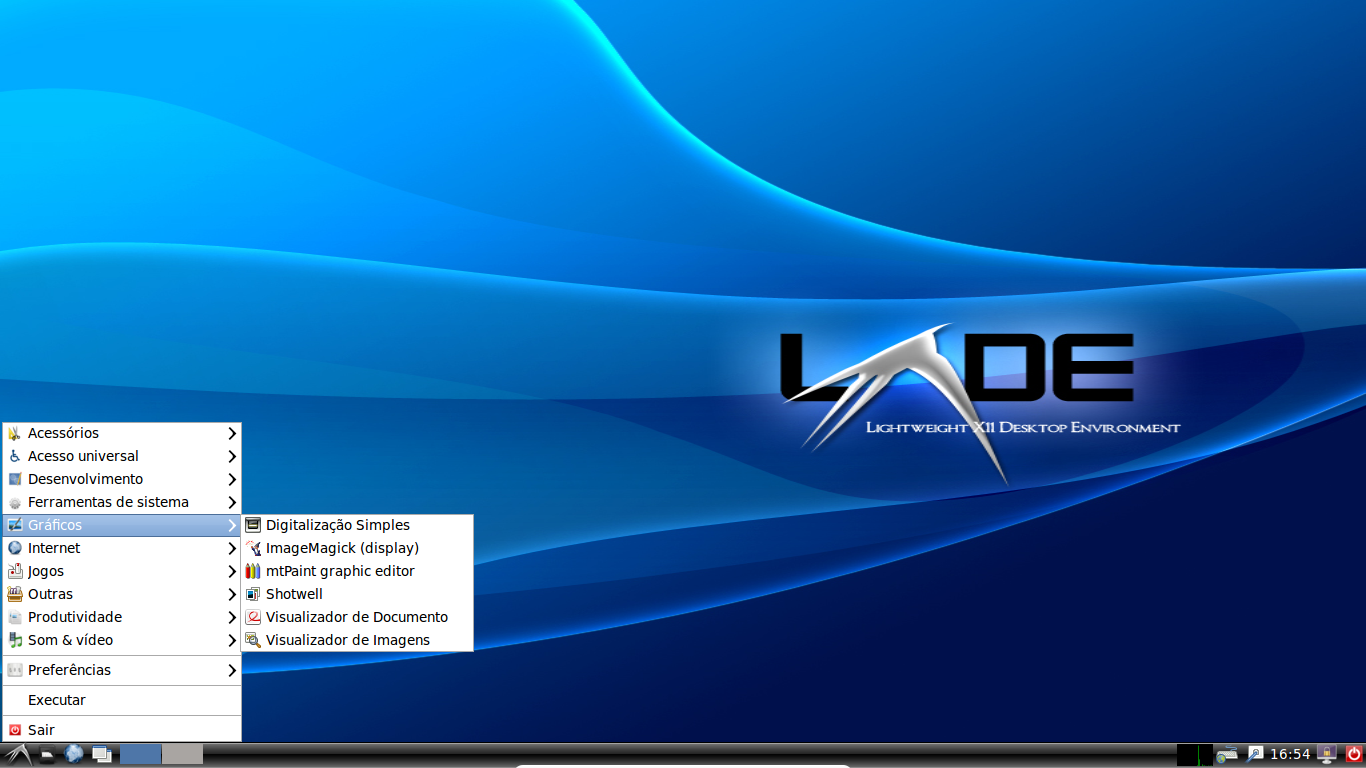
\includegraphics[scale=0.3]{lxde.png}
 \caption{Ambiente LXDE, onde pode ser visto o menu dividido por áreas.}
 \label{lxde}
\end{figure}

Para além do famoso \textit{PCManFM} (\autoref{pcmanfm}), o LXDE não apresenta muitas aplicações nativas no seu sistema, principalmente para não consumir demasiado espaço \cite{AplicacoesLXDE}. Ainda assim, salientamos o \textit{Leafpad}, um editor de texto bastante leve, e \textit{Openbox}, o gestor de janelas.

\begin{figure}
 \center
 \includegraphics[scale=0.3]{pcmanfm.png}
 \caption{Gestor de ficheiros PCManFM.}
 \label{pcmanfm}
\end{figure}

Nos nossos testes, o LXDE utilizou uma quantidade de memória Ram bastante baixa (processo \textit{lxpanel} (\autoref{memlxde}), aproximadamente 20 Mb), o que justifica a sua fama de sistema extremamente leve. Também no CPU obteve bons resultados, ficando-se pelos 0,3\%.

\begin{figure}
 \center
 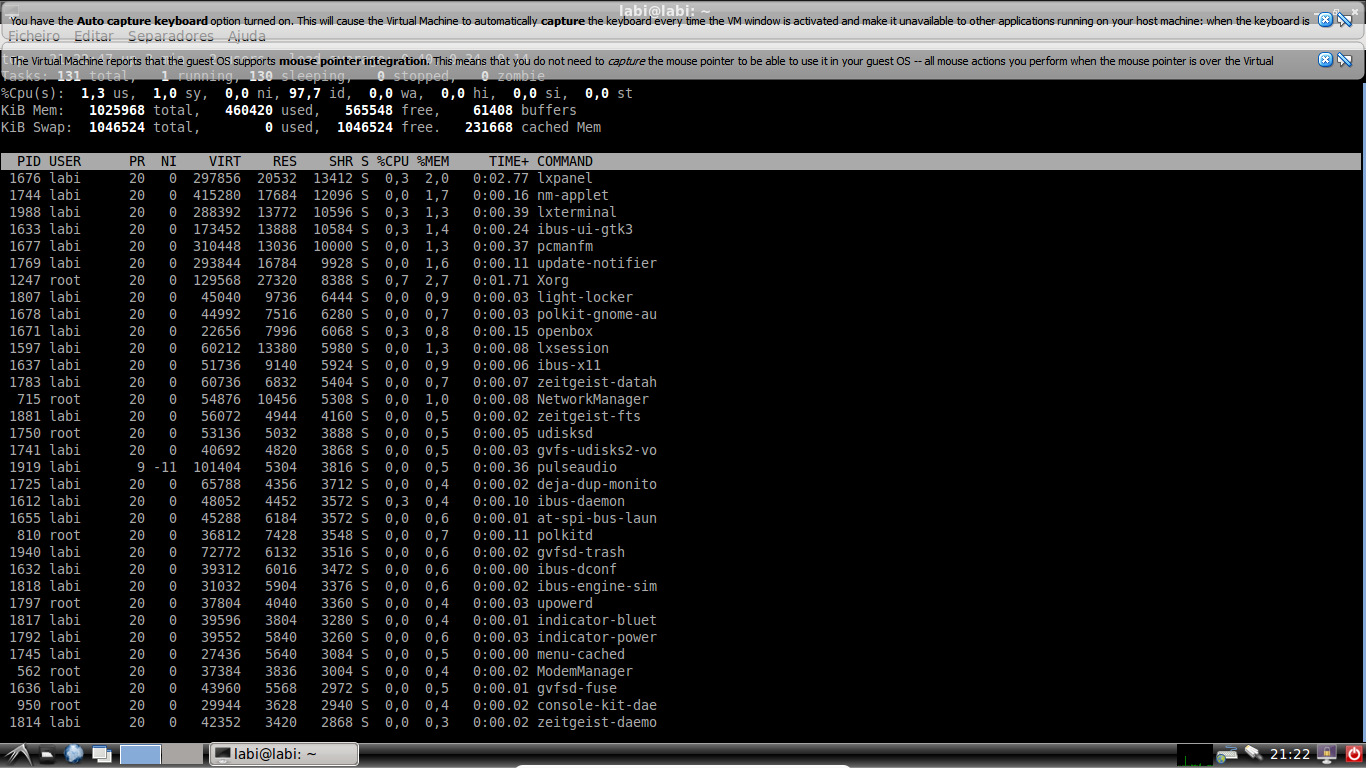
\includegraphics[scale=0.3]{memlxde.png}
 \caption{Gestão de memória no Sistema LXDE. O processo de onde foram retirados os dados foi o primeiro, \textit{lxpanel}.}
 \label{memlxde}
\end{figure}


\chapter{E17}

\paragraph{  }E17, Enlightenment ou E, é uma interface gráfica que foi criada em 1997 por \textit{"Rasterman"}, engenheiro de software na Universidade da Carolina do Norte \cite{E17}. E17 diferencia-se dos restantes ambientes por ser independente, ou seja, tem as suas bibliotecas, serviços e aplicações próprias.

É alvo de bastantes críticas devido à sua interface completamente diferente de todos os outros sistemas, tornando-se menos intuitivo ao utilizador experienciado em Linux regular \cite{CriticasE17}. No entanto, tem um aspeto bastante inovador e apelativo a quem procura diversidade gráfica.

A comunidade deste sistema é bastante extensa, pois há defensores acérrimos deste sistema (embora também haja o contrário) \cite{CriticasE17}. Os seus repositórios podem ser encontrados no link \url{https://git.enlightenment.org/}.

A interface do E17 é a menos ordinária das analisadas (\autoref{E17}). Contém um barra inferior horizontal apenas a meio do ecrã com aplicações definidas pelo utilizador, ao lado da indicação da memória Ram usada e memória em cache da placa gráfica. Ao lado, temos também a indicação do horário, do som e dos ambientes. Do outro lado, temos o seu menu (\autoref{E172}).

\begin{figure}
 \center
 \includegraphics[scale=0.3]{E1.png}
 \caption{Ambiente E17.}
 \label{E17}
\end{figure}

\begin{figure}
 \center
 \includegraphics[scale=0.3]{E2.png}
 \caption{Menu do ambiente E17, onde pode ser vista a barra inferior alguns os ícones de aplicações.}
 \label{E172}
\end{figure}

Com um simples clique no ecrã temos acesso ao menu com todas as aplicações, ficheiros e definições de sistema. De notar que é um ambiente totalmente configurável, portanto o aspeto poderá ser bastante diversificado de utilizador para utilizador.

O E17 não tem aplicações pré-instaladas a destacar, para além do seu inovador gestor de janelas \textit{Enlightment} (\autoref{E17}). Apresentou resultados muito razoáveis no consumo de memória Ram (Processo Enlightment (\autoref{mem17})). Consumiu sempre perto de 45 Mb, como pode ser visto pelo processo \textit{enlightenment}. Também o consumo de CPU se manteve nos 5\%, um resultado não muito baixo, mas aceitável quando comparado com os ambientes vistos.

\begin{figure}
 \center
 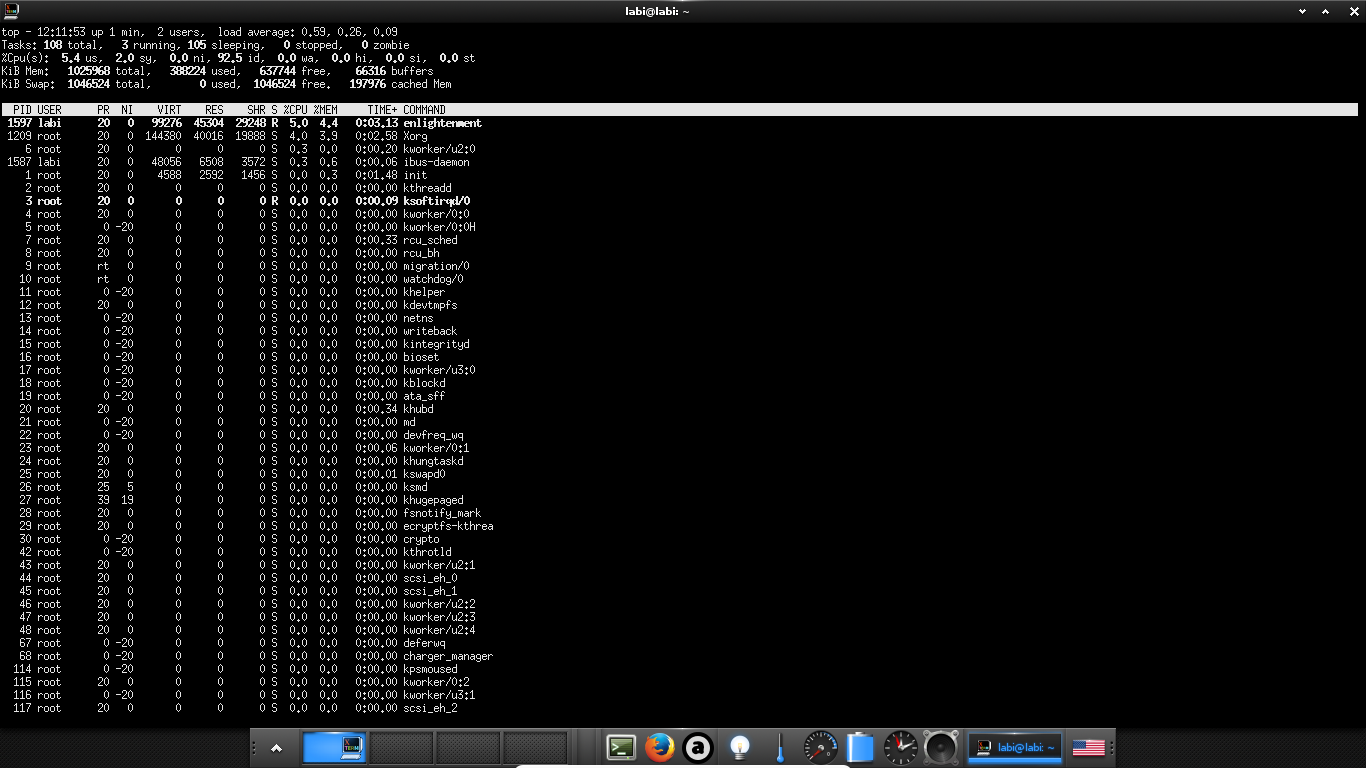
\includegraphics[scale=0.3]{memenl.png}
 \caption{Memória Ram usada pelo sistema. Os dados foram retirados do primeiro processo, o\textit{ enlightenment}.}
 \label{mem17}
\end{figure}


\chapter{XFCE4}

\paragraph{  }Criado em 1996 por Olivier Fourdan, \textit{XFCE4} é um ambiente gráfico baseado nas plataformas \textit{Unix-like} \cite{XFCE4}. O seu objetivo inicial era ser rápido e leve, mantendo um aspeto gráfico minimamente apelativo e agradável.

Nos últimos anos, devido às bibliotecas oferecidas, é maioritariamente usado como sistema para o ensino de programação em C/C++, Phyton e Perl, podendo até ser usado no campo da programação profissional. XFCE4 tem os seus repositórios em \url{http://git.xfce.org/}. Não é das maiores comunidades, assemelhando-se em número de colaboradores à do ambiente LXDE (anteriormente visto).

Como foi desenhado para ser um sistema extremamente leve, não apresenta menus com grandes animações. Ainda assim, apresenta duas barras (\autoref{xfce4}): uma superior e uma inferior.

\begin{figure}
 \center
 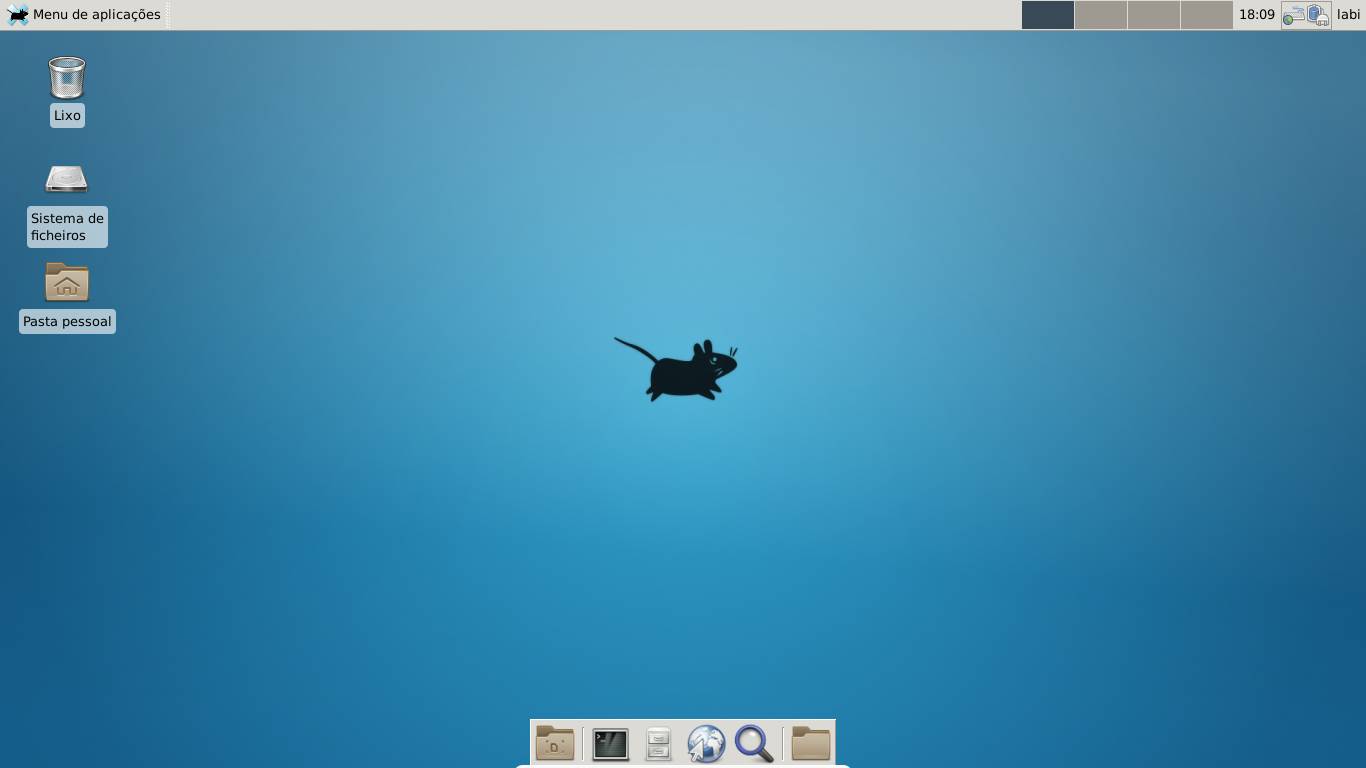
\includegraphics[scale=0.3]{xfce.png}
 \caption{Ambiente XFCE4. Apresenta duas barras: Uma inferior e uma superior}
 \label{xfce4}
\end{figure}

A barra inferior dá acesso rápido às aplicações mais usadas, ou definidas pelo utilizador.

A barra superior, do lado direito, para além das definições do sistema e das horas, tem o menu dos ambientes virtuais. Do lado esquerdo tem o menu de aplicações, que dá acesso a todas as aplicações instaladas no sistema (\autoref{xfce42}).

\begin{figure}
 \center
 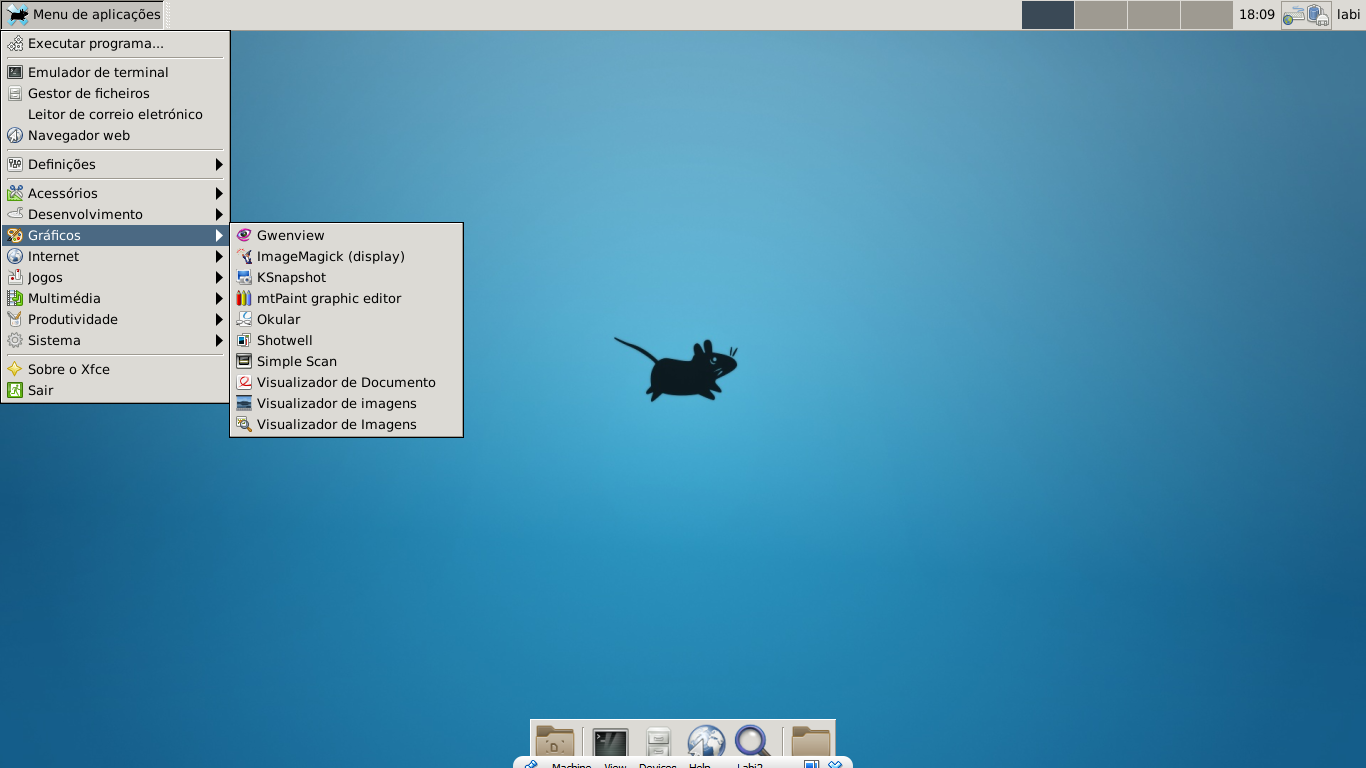
\includegraphics[scale=0.3]{xfce2.png}
 \caption{Barra lateral do XFCE4}
 \label{xfce42}
\end{figure}

O XFCE4 vem com um pacote interessante de aplicações. O \textit{Thunar}, gestor de ficheiros, é bastante simples e rápido de usar. O mesmo se pode constatar do browser \textit{Midory} \cite{AplicacoesXFCE4}.

O \textit{Xfburn} e \textit{Xfmedia} são aplicações criadas especificamente para o XFCE. O primeiro é um gravador de DVD's, CD's e ficheiros .ISO e o segundo é o \textit{media player} do sistema. Todos são softwares bastante robustos, com o objetivo de sobrecarregar ao mínimo os recursos do computador.

Por fim, existe ainda o \textit{Ristretto}, um dos melhores visualizadores de imagens para Linux.

A interface apresenta um consumo de memória Ram baixo, com aproximadamente 20Mb usados, tal como o ambiente LXDE visto anteriormente (processo \textit{Xfdesktop} (\autopageref{memxfce})). Também exige bastante pouco de CPU, consumindo apenas 0,3\%.

\begin{figure}
 \center
 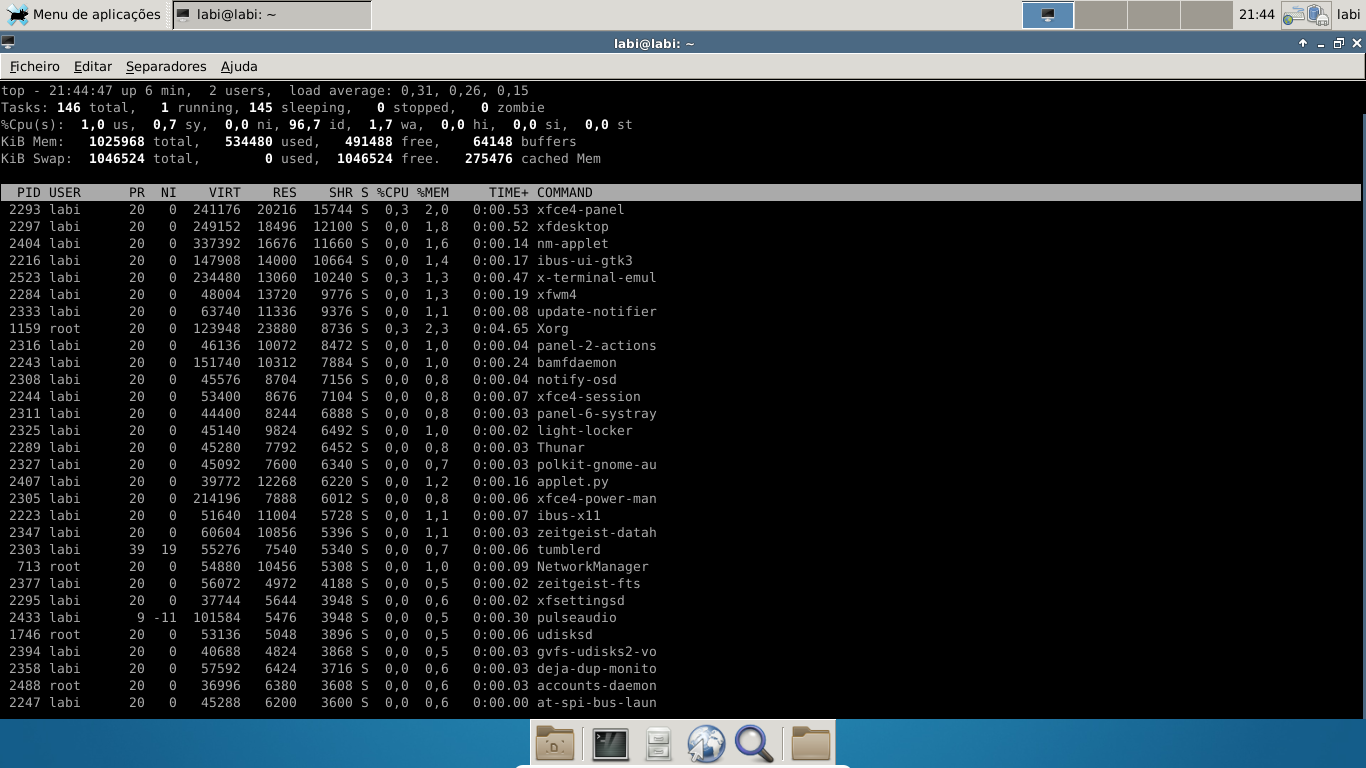
\includegraphics[scale=0.3]{memxfce.png}
 \caption{Consumo de memória do XFCE4. Dados retirados do segundo processo, \textit{xfdesktop}.}
 \label{memxfce}
\end{figure}



\chapter{xmonad}

\paragraph{  }\textit{xmonad} é um gestor de janelas escrito em \textit{Haskell}. O projeto é recente, iniciado em 2007, e tem como principal vantagem a facilidade de uso, especialmente no alinhamento das janelas abertas \cite{Xmonad}.

Todas as funcionalidades estão disponíveis apenas com o teclado, sendo dispensável o uso do rato. Podem ser ainda aplicados temas diferentes a ecrãs virtuais diferentes.

De entre os sistemas testados, é o que apresenta uma menor comunidade. Os seus repositórios podem ser encontrados em \url{http://code.haskell.org/xmonad/}. No entanto, justifica-se devido a ser um gestor de janelas, não uma interface gráfica. Logo, necessita de muito menos recursos e de menos atualizações de versões anteriores.

O xmonad é um gestor de janelas completamente diferente do que foi visto até agora (\autoref{Xmonad}). Não é uma interface gráfica, pelo que pode ser controlada apenas com o teclado. À primeira vista, pode não ser visualmente apelativo pois é minimalista, mas pode trazer bastantes vantagens para os utilizadores experientes que desejam efetuar tarefas de maneira rápida, simples e eficiente.

\begin{figure}
 \center
 
\includegraphics[scale=0.3]{xmonad.png}
 \caption{Ambiente \textit{xmonad}. Como pode ser visto, não apresenta qualquer barra ou menu, apenas o Wallpaper.}
 \label{Xmonad}
\end{figure}

Como é apenas um gestor de janelas, não tem quaisquer aplicações instaladas.

Como esperado, foi o resultado o mais baixo no nosso teste, nunca ultrapassando 4 Mb sempre que foi usado (Processo\textit{ Xmonad}, (\autoref{Xmonadmem})). No entanto, é preciso reconhecer que é apenas um gestor de janelas, logo não oferece uma interface gráfica tão completa como os já testados anteriormente. Destaca-se pela sua estabilidade e rapidez de execução, como também mostra o consumo de CPU, que nem chega a ser contabilizado de tão ínfimo que é.

\begin{figure}
 \center
 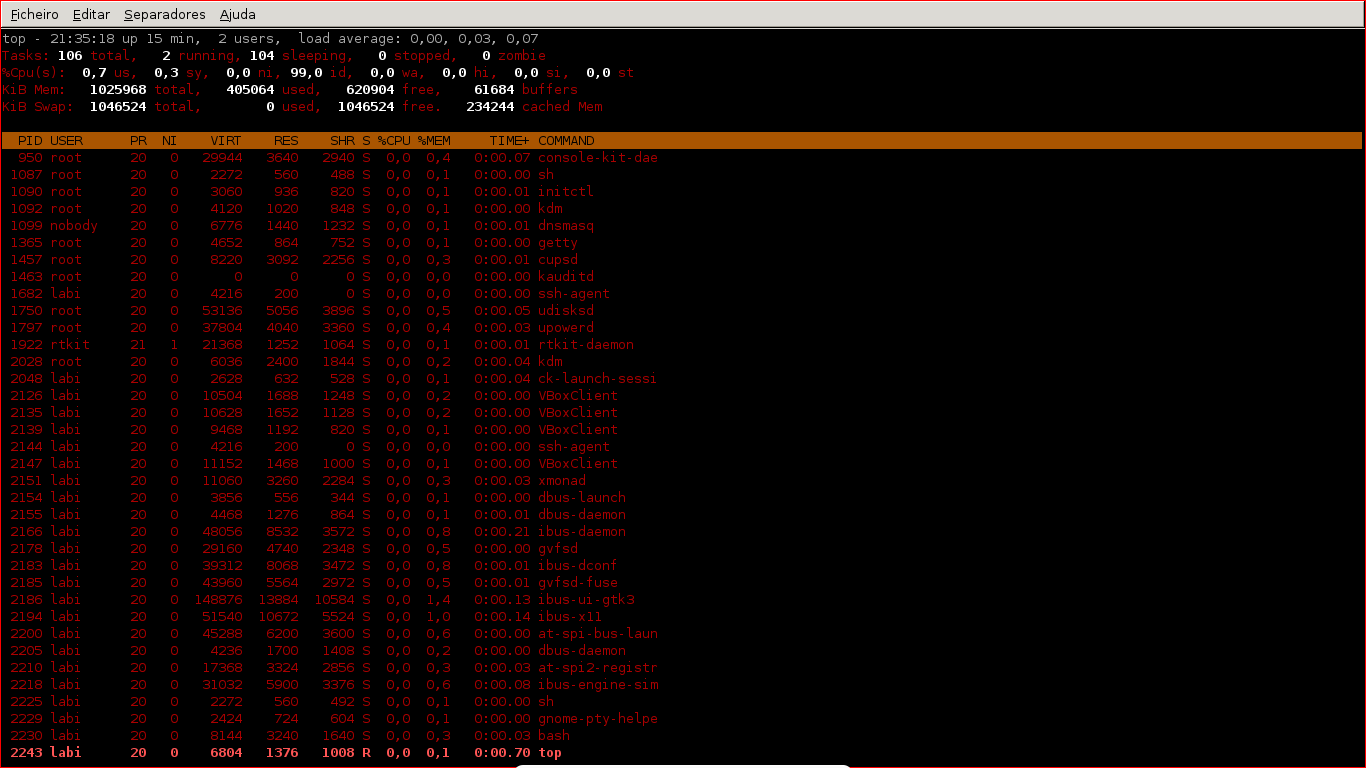
\includegraphics[scale=0.3]{memx.png}
 \caption{Gestão de memória do ambiente \textit{xmonad}. O processo a ser visto é o\textit{ xmonad}, ligeiramente abaixo do centro do ecrã.}
 \label{Xmonadmem}
\end{figure}

\chapter{awesome}

\paragraph{  }O gestor de janelas \textit{awesome} foi criado em 2007, baseado na personagem de \textit{How I Met Your Mother}, \textit{Barney Stinson}. Tem como objetivo ser rápido e leve, mas personalizável usando apenas o teclado \cite{Awesome}.

Foi desenhado para utilizadores avançados, desenvolvedores ou profissionais que necessitam de realizar tarefas com algum poder computacional.

Tal como a comunidade de \textit{xmonad}, a de \textit{awesome} também não é muito extensa. Os seus repositórios podem ser encontrados em \url{https://github.com/awesomeWM/awesome}.

\textit{awesome} também foi desenvolvido tendo como base uma ideia diferente de ambiente gráfico (\autoref{Awesome}). Como tal, é bastante simples, apresentando apenas uma barra lateral superior simplista com nove ecrãs virtuais e um menu iniciar bastante rudimentar (\autoref{Awesomem}).

\begin{figure}
 \center
 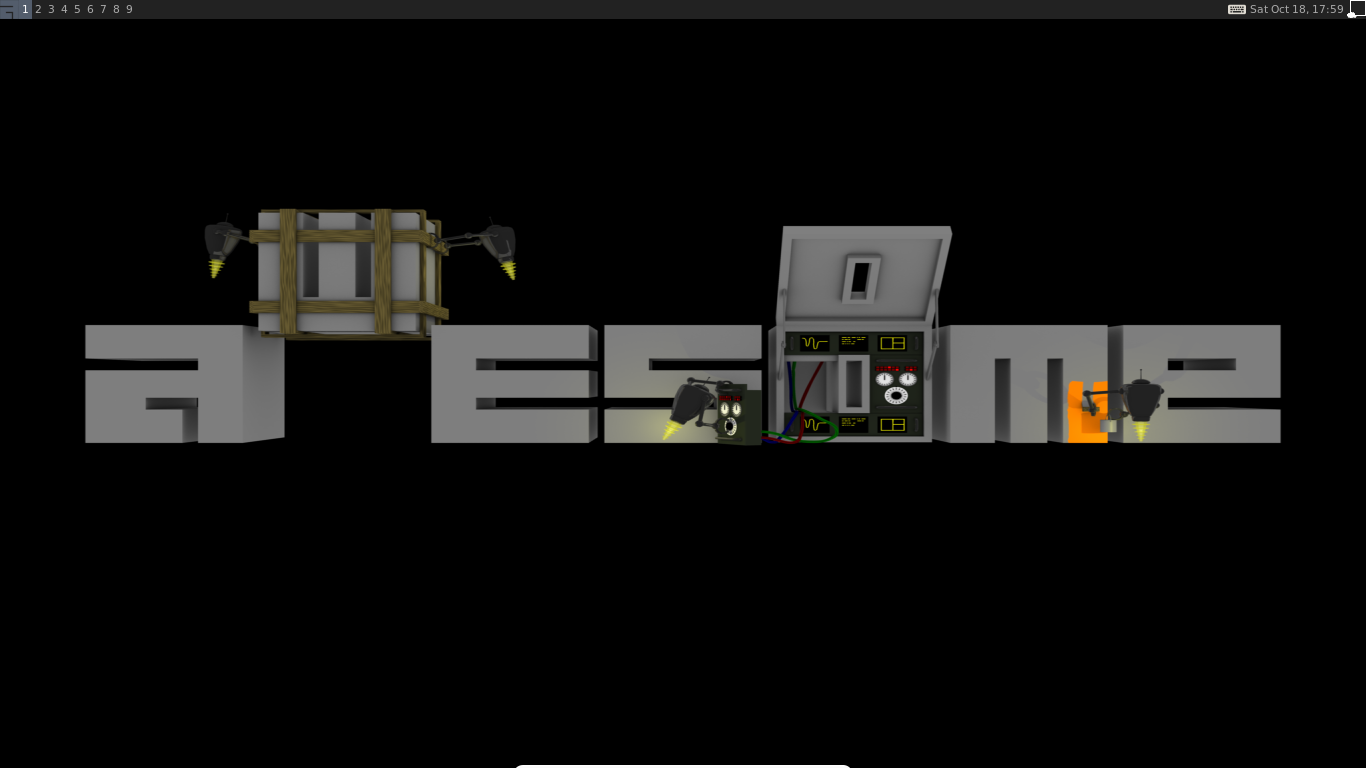
\includegraphics[scale=0.3]{aw1.png}
 \caption{Ambiente\textit{ awesome}.}
 \label{Awesome}
\end{figure}

\begin{figure}
 \center
 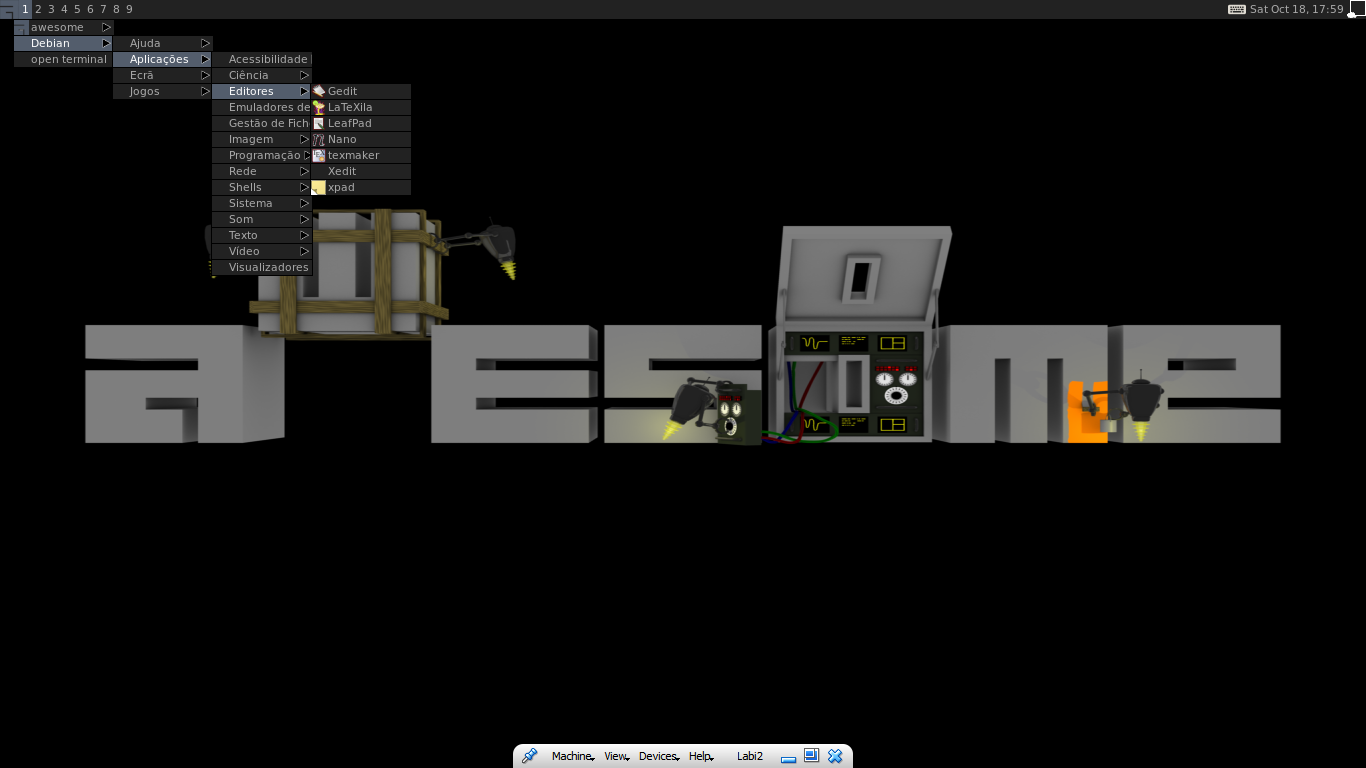
\includegraphics[scale=0.3]{aw2.png}
 \caption{Menu do Ambiente \textit{awesome}.}
 \label{Awesomem}
\end{figure}

Não traz aplicações instaladas visto que é um gerenciador de janelas. O impacto na memória também é diminuto, tal como o\textit{ xmonad}. Nos nossos testes, dispendeu uma memória Ram de aproximadamente 8 Mb (como podemos ver no processo \textit{awesome}) (\autoref{Awesomemo}), o que é bastante diminuto. No entanto, o consumo de CPU já é surpreendentemente elevado, atingindo 4,3\%.

\begin{figure}
 \center
 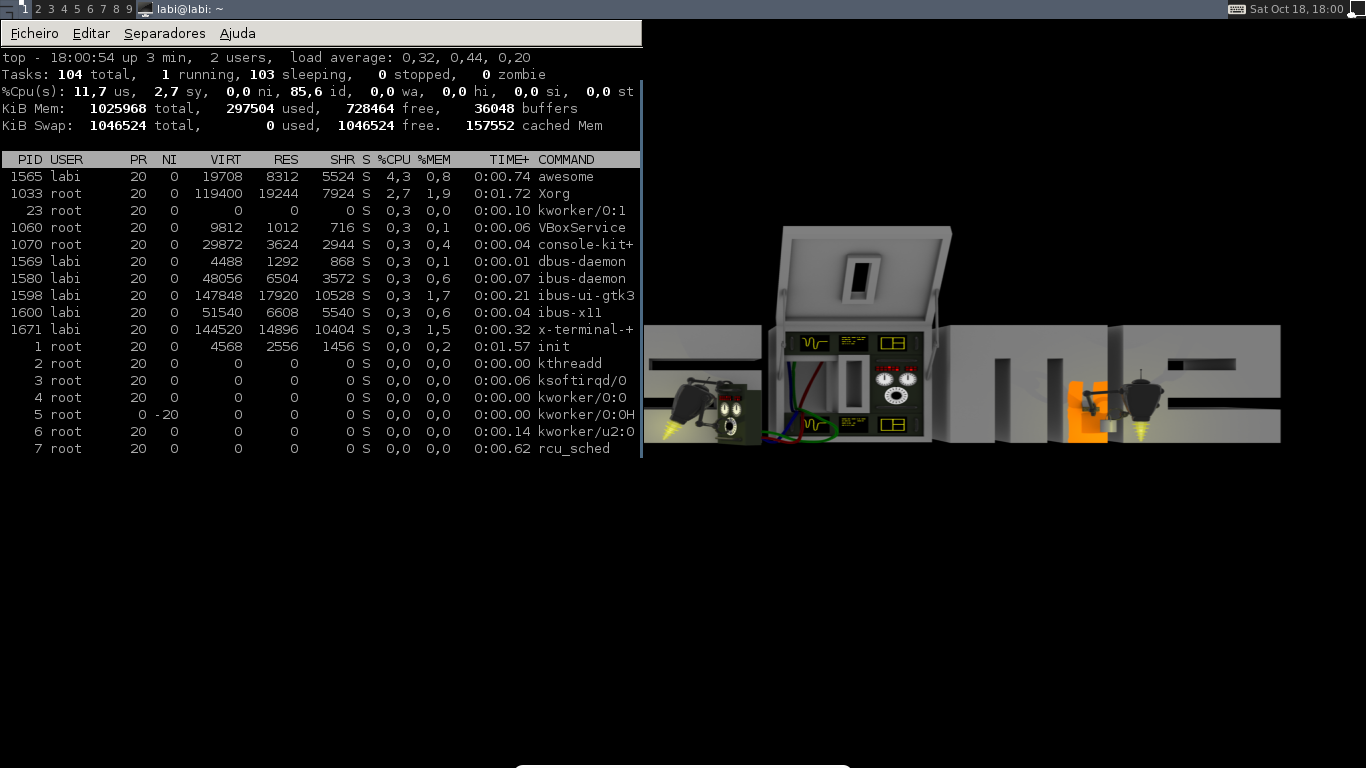
\includegraphics[scale=0.3]{memaw.png}
 \caption{Gestão de memória \textit{awesome. } Os dados foram retirados do primeiro processo, \textit{awesome.}}
 \label{Awesomemo}
\end{figure}

\part{Conclusões}

\chapter{Conclusão}
\paragraph{  }Neste trabalho tentámos descrever alguns ambientes gráficos para Linux, sem detalhar demasiado a análise, abordando apenas as suas linhas gerais. Usámos todos os ambientes gráficos descritos, apenas durante o período de tempo disponível para a realização do trabalho, o que não permitiu ter análises mais detalhadas. No entanto, todos os \textit{screenshots} e análises de memória foram feitos totalmente por nós.

É possível termos cometido alguns erros, especialmente na referência às aplicações e à memória consumida pelos ambientes. Nas aplicações, apenas as referimos com base na pesquisa feita, derivado do pouco tempo disponível. Quanto à memória, como os ambientes foram instalados em máquinas virtuais, é possível que os resultados não sejam totalmente confiáveis. Poderemos também estar suscetíveis a outros erros de leitura nos terminais testados.

Também é possível termos introduzido alguma subjetividade quando falámos sobre os ambientes gráficos. Tentámos evitar ao máximo, mas somos apaixonados por estes assuntos, temos ambientes favoritos e outros não tanto, e esperamos não ter deixado transparecer nada que possa induzir o leitor em erro.


\bibliography{bib}
\bibliographystyle{plain}

\end{document}